\documentclass[12pt,a4paper]{report}

% ============================================================================
% PACKAGES & SETUP
% ============================================================================
\usepackage[english]{babel}
\usepackage[margin=2.5cm]{geometry}
\usepackage{mathptmx}          % Times New Roman equivalent
\usepackage{setspace}
\usepackage{graphicx}
\usepackage{fancyhdr}
\usepackage{tcolorbox}
\usepackage{hyperref}
\usepackage{xcolor}
\usepackage{listings}
\usepackage{float}
\usepackage{array}
\usepackage{booktabs}
\usepackage{amsmath}
\usepackage{amssymb}
\usepackage{tikz}
\usetikzlibrary{patterns}
\usepackage{svg}
\usepackage{subcaption}
\usepackage{xspace}

% Line spacing
\setstretch{1.15}

% Paragraph indentation
\parindent=0.5cm

% Page number setup
\pagestyle{fancy}
\fancyhf{}
\rfoot{\thepage/\pageref{LastPage}}
\renewcommand{\headrulewidth}{0pt}
\renewcommand{\footrulewidth}{0.4pt}

% Hyperref colors
\hypersetup{colorlinks=true, linkcolor=black, urlcolor=blue}

% Chapter formatting
\usepackage{titlesec}
\titleformat{\chapter}[display]
  {\normalfont\bfseries\fontsize{18}{20}\selectfont}
  {Chapter \thechapter}{0.5cm}{}
\titleformat{\section}
  {\normalfont\bfseries\fontsize{14}{16}\selectfont}
  {\thesection}{0.5cm}{}
\titleformat{\subsection}
  {\normalfont\bfseries\fontsize{12}{14}\selectfont}
  {\thesubsection}{0.5cm}{}

% Last page reference
\usepackage{lastpage}
\usepackage{pdfpages}

% ============================================================================
% DOCUMENT BEGIN
% ============================================================================
\begin{document}

% ============================================================================
% COVER PAGE
% ============================================================================

\includepdf[pages=-]{Page_Garde.pdf}


% ============================================================================
% ACKNOWLEDGEMENTS
% ============================================================================
\chapter*{Acknowledgements}
\addcontentsline{toc}{chapter}{Acknowledgements}

I want to start by thanking Ahmed Ferchichi, my corporate supervisor. He believed in this project from day one and gave me the freedom to experiment. His feedback helped me navigate the tricky architectural decisions and focus on what actually matters in a real production environment. 

Syrine Karoui, my academic supervisor, was a massive help in organizing my thoughts. She pushed me to connect the deep technical work back to the original problem statement, which really changed how I approach engineering documentation.

I also want to thank the entire team at Monetique. They didn't treat me like an intern doing busywork. They reviewed my code seriously, discussed trade-offs, and shared their experience freely. 

On a personal note, I couldn't have done this without my family, who supported me through every late night of debugging and every stressful deadline. Most of all, a heartfelt thank you to my fiancée. Your love, patience, and unwavering belief in me have been my greatest support throughout this entire journey. Thank you for always listening to my ideas, comforting me when things got difficult, and celebrating every breakthrough by my side. You kept me motivated when the code wouldn't compile and the solutions felt out of reach. This accomplishment is as much yours as it is mine, and I am incredibly grateful to share it with you.

\newpage

% ============================================================================
% TABLE OF CONTENTS
% ============================================================================
\tableofcontents
\newpage

\listoffigures
\addcontentsline{toc}{chapter}{List of Figures}
\newpage

\listoftables
\addcontentsline{toc}{chapter}{List of Tables}
\newpage

% ============================================================================
% GENERAL INTRODUCTION
% ============================================================================
\chapter*{General Introduction}
\addcontentsline{toc}{chapter}{General Introduction}

\section*{Context and Motivation}

Modern enterprise infrastructure has become increasingly complex. Organizations manage multiple environments (production, staging, development), distributed microservices, containers, virtual machines, and cloud resources spanning regulatory boundaries. In the financial services and payments sector (the \textit{monetique} domain), this complexity is compounded by reliability requirements: any infrastructure failure directly impacts revenue, customer trust, and regulatory compliance.

Traditional infrastructure monitoring approaches suffer from significant limitations:

\begin{itemize}
  \item \textbf{Tool Fragmentation}: Separate platforms for metrics (Prometheus), logs (ELK stack), alerts (Alertmanager), and incidents create disparate systems that operators must manually correlate.
  \item \textbf{Manual Provisioning}: Adding a new node for monitoring requires deep DevOps expertise—SSH key management, Ansible inventories, Prometheus targets, and logging agent configuration are often error-prone and time-consuming.
  \item \textbf{Lack of Intelligence}: Operators spend hours correlating logs, metrics, and alerts to understand root causes. AI-driven analysis is rare in traditional stacks.
  \item \textbf{Access Control Challenges}: Most monitoring platforms offer only coarse-grained RBAC, making it difficult to enforce environment-level data isolation in multi-tenant scenarios.
  \item \textbf{Deployment Tracking Gap}: CI/CD systems operate independently from observability, leaving operators without visibility into what was deployed and when.
\end{itemize}

\section*{Problem Statement}

This project addresses a critical set of operational bottlenecks within the department's infrastructure operations:

\begin{enumerate}
  \item \textbf{Prolonged Incident Diagnosis:} Operators face an extensive investigation window, historically averaging 45 minutes, to identify the root cause of failures.
  \item \textbf{Observability Tool Fragmentation:} Metrics, logs, alerts, and deployment records reside in disconnected systems, requiring operators to manually switch context and correlate disparate data.
  \item \textbf{Inefficient Node Provisioning:} Onboarding new infrastructure nodes for monitoring is a slow, error-prone manual process that takes approximately 8 to 10 hours per node.
  \item \textbf{Lack of Data Correlation:} The lack of automated correlation between time-series metrics and full-text log files hinders quick detection of systemic anomalies.
  \item \textbf{Coarse Access Isolation:} Existing monitoring tools do not support environment-level data segregation, which presents a significant security risk for multi-tenant deployments.
  \item \textbf{Inconsistent Agent Configuration:} Monitoring agents deployed across heterogeneous nodes suffer from configuration drift, as each node is provisioned manually with no centralized template enforcement.
  \item \textbf{Absence of Deployment-to-Incident Traceability:} CI/CD pipeline events are not linked to the observability layer, preventing operators from correlating a new release with a subsequent service degradation.
  \item \textbf{Risky Container Operations:} No visual interface for container lifecycle management, forcing operators to rely on risky direct SSH access to debug deployed stacks.
  \item \textbf{Unsecured Image Registry:} No private registry enforcing image vulnerability scanning before a container reaches production.
  \item \textbf{Static Credentials Storage:} Secrets and credentials handled as static, disk-based configuration rather than dynamically injected at runtime.
\end{enumerate}

\section*{Project Objectives}

The \textbf{Monetique Eye} project was structured to deliver an enterprise-grade observability platform through multiple sequential phases, each building upon the previous:

\begin{description}
  \item[Phase 1: Backend Foundation \& Security] Establish a secure, scalable data layer with JWT authentication, RBAC, and a comprehensive 25-entity data model.
  \item[Phase 2: Core UI \& Dashboarding] Build a React-based frontend with environment management, real-time monitoring dashboards, and an interactive topology visualization.
  \item[Phase 3: Advanced Observability Features] Implement log aggregation, real-time log search, and the AI-powered « Root Cause Intelligence » engine.
  \item[Phase 4: Operational Intelligence] Create executive dashboards with AI-generated summaries, stability scoring, and operational signal detection.
  \item[Phase 5: DevSecOps \& CI/CD Integration] Integrate Jenkins pipelines, Portainer for container management, implement automated deployment tracking, and harden security with Vault, Falco, and Harbor.
\end{description}

\section*{Chapter Overview}

This report documents the complete internship experience and the development of Monetique Eye:

\begin{itemize}
  \item \textbf{Chapter 1} presents the company context, the department, the problem statement, the critique of existing systems, the project scope, and the methodology and planning that governed development.
  
  \item \textbf{Chapter 2} details the proposed architecture and technical design, covering high-level architecture, the five-phase roadmap, key design principles, data models, and deployment topologies.
  
  \item \textbf{Chapter 3} describes the core platform realization, presenting the implementation of Phases 1 through 4 from the backend and security foundation to operational intelligence features.
  
  \item \textbf{Chapter 4} addresses the DevSecOps integration, pipeline configurations, and project outcomes, including implementation challenges, scale, and performance metrics.
\end{itemize}

This report avoids raw code listings in the main text; technical implementation details and code snippets are deferred to the appendices. The focus is on \textbf{why} design choices were made and \textbf{how} they address the original problem.

\newpage

% ============================================================================
% CHAPTER 1: CONTEXT, ANALYSIS AND PROPOSED SOLUTION
% ============================================================================


\chapter{Company Context and Project Specification}

\section*{Introduction}
\addcontentsline{toc}{section}{Introduction}
This chapter establishes the organizational and operational environment of the host company, focusing on the specific infrastructure challenges that motivated this work. We analyze the existing observability tooling, identify key operational limitations, and define the scope and feasibility boundaries of the project. Finally, we detail the engineering methodology and project timeline that structured the development lifecycle.

\section{Company Overview}

Monetique is a leading finance software company specializing in digital payment solutions and infrastructure services for the financial sector. The company manages critical payment processing systems, transaction platforms, and enterprise middleware for financial institutions and retailers.

The infrastructure and platform division where this internship took place is responsible for keeping Monetique's own systems running. Multiple internal teams (Infrastructre, E-commerce, dev, operations) manage different environments and clusters, each with their own monitoring needs. The goal of this internship was to build an internal observability DevOps platform that these teams could all use, rather than each team cobbling together their own fragmented tooling.

\section{The Department: Infrastructure \& Observability}

The internship was embedded within the \textbf{Infrastructure and Observability} department, a team of approximately 20 engineers responsible for:

\begin{itemize}
  \item Designing and operating the company's private cloud platform
  \item Managing multi-environment deployments (production, staging, development)
  \item Implementing monitoring and alerting infrastructure
  \item Providing operational support (24/7 on-call rotations for critical systems)
  \item Building internal tools for DevOps automation
\end{itemize}

The department already operated a fragmented observability stack: Prometheus for metrics, Elasticsearch for logs, Grafana for visualization, and Ansible for infrastructure automation etc ... However, no unified platform existed to tie these tools together—operators still performed manual correlation and root cause analysis.

\section{Initial Problem Statement}

At the start of the internship, the team articulated a specific pain point:

During an incident, operators historically faced an extensive investigation window: they manually SSH into servers, grep logs, run ad-hoc Prometheus queries, and correlate events across multiple dashboards. By the time they've diagnosed the root cause, customer impact has already accumulated. We needed a unified observability platform with intelligent diagnostics to significantly cut incident resolution time.

Additionally, provisioning new monitoring infrastructure was slow: adding a client node for monitoring required a DevOps engineer to manually configure SSH keys, Ansible inventories, Prometheus targets, and logging agents—a process that typically took roughly 4 hours per node.

\section{Study and Critique of the Existing System}

Prior to this project, the infrastructure and platform division relied on a collection of independent, best-of-breed open-source components, each addressing a narrow operational concern. A time-series database handled metric collection and numeric health indicators with high reliability. A separate full-text search engine aggregated and indexed application logs, enabling rapid keyword-based retrieval. A visualization layer rendered dashboards from the metric store, while a configuration management framework orchestrated infrastructure changes through declarative automation.

Although each component excels within its intended scope, the absence of a unifying orchestration layer introduced four categories of operational friction. First, the tools operated as isolated data silos: correlating a resource utilization anomaly in the metric store with a corresponding error pattern in the log index required operators to manually extract timestamps from one interface and re-enter them into another—a tedious, error-prone process during time-critical incidents. Second, provisioning new infrastructure nodes for monitoring demanded sequential manual intervention across multiple subsystems—credential distribution, host inventory registration, metric target declaration, and log agent configuration—resulting in a per-node onboarding cost measured in hours rather than minutes. Third, the platform's access control model was coarse-grained and tool-scoped: permissions were granted at the level of the entire monitoring system rather than at the granularity of individual environments, which prevented the strict data isolation required in multi-tenant financial deployments. Fourth, no mechanism existed to link deployment pipeline events with observability data, leaving operators unable to trace a service degradation back to a specific release.

The comparison in Table~\ref{tab:existing_critique} highlights the functional gaps between the existing tooling and the operational requirements of the organization.

\begin{table}[H]
\centering
\renewcommand{\arraystretch}{1.3}
\begin{tabular}{|l|p{6cm}|p{6cm}|}
\hline
\textbf{Capability} & \textbf{Existing Approach} & \textbf{Required Capability} \\
\hline
Incident Diagnosis & Manual terminal investigation and log grepping. & Automated root-cause correlation and diagnostic suggestions. \\
\hline
Node Provisioning & Manual configuration of inventories, keys, and agents (4+ hours). & Idempotent, automated agent deployment (2-3 minutes). \\
\hline
Log/Metric Correlation & Separated silos; manual timestamp alignment. & Dynamic, automated correlation in a unified view. \\
\hline
RBAC Granularity & Coarse-grained, tool-wide permissions. & Strict, environment-scoped role-based access control. \\
\hline
AI Analysis & Absent; manual diagnosis based on experience. & AI-assisted operational digests and pattern detection. \\
\hline
Deployment Tracking & Separated CI/CD pipelines; no observability links. & Integrated deployment timelines linked to incident analysis. \\
\hline
\end{tabular}
\caption{Comparison of Existing Approach vs. Required Capability}
\label{tab:existing_critique}
\end{table}

This critique demonstrates that the department does not require a replacement of its existing technical stack, but rather a unified orchestration and intelligence layer that integrates these systems to eliminate manual effort and enforce compliance.

\section{Scope and Feasibility}

Given a six-month internship window, the team and I agreed on the following scope:

\begin{itemize}
  \item Build a full-stack application (backend API + React UI + MySQL database)
  \item Automate infrastructure provisioning through a one-click deployment interface that covers container lifecycle handoff to Portainer, registry gating through Harbor, and secrets injection via Vault at deployment time
  \item Integrate the existing Prometheus, Elasticsearch, and Ansible stack (no replacement)
  \item Implement RBAC and multi-environment isolation
  \item Add AI-powered log analysis using a large language model API
  \item Provide enough flexibility for future enhancements (phases 6 and beyond)
  \item Add container lifecycle visibility via Portainer.
  \item Enforce image scanning and registry gating via Harbor.
  \item Centralize secrets management via Vault.
\end{itemize}

Out of scope (deferred to future phases):
\begin{itemize}
  \item Kubernetes-native deployment (only Docker + VMs in scope)
  \item Custom machine learning model training
  \item Advanced predictive analytics
\end{itemize}

\section{Perspectives and Future Evolution}

While the defined internship scope addresses the department's most pressing operational gaps, three longer-term evolution trajectories have been identified to guide the platform's growth beyond the current development cycle.
\begin{enumerate}
    \item \textbf{Future Objective 1 - Kubernetes / cloud-native cluster support}: Moving from Docker Compose to Helm charts (future-proofing).
    \item \textbf{Future Objective 2 - Multi-tenant SaaS evolution}: Isolated namespaces per organization within the data model.
    \item \textbf{Future Objective 3 - Advanced ML-based predictive anomaly detection}: Moving from rule-based to model-based alerting.
\end{enumerate}

These future steps will culminate in a unified observability platform where metrics, logs, alerts, and incidents are in one place, with automated one-click node provisioning for both containerized and standalone Linux nodes, full Jenkins CI/CD integration, and AI-powered operational intelligence.

\section{Methodological \& Technological Choices}

\subsection{Tools Justification}

The technology stack was carefully selected to balance rapid development, enterprise-grade reliability, and alignment with modern DevOps practices.

\subsubsection{Backend}
The backend layer is built using the Spring Boot framework on Java 21, incorporating Hibernate as the object-relational mapping tool, Liquibase for database schema migration, and Spring Security for request lifecycle protection. The choice of a mature, multithreaded ecosystem is dictated by the deeply relational nature of the 28 core system entities, which require strict ACID compliance and foreign key enforcement to guarantee data integrity across environments. Java 21's support for high-concurrency virtualization allows the API to process multiple telemetry feeds and orchestrate concurrent node deployments without thread exhaustion, matching the strict reliability demands of a financial services environment.

\subsubsection{Frontend}
The user interface is developed as a single-page application using React 19, TypeScript, and Vite, with Tailwind CSS for styling, React Flow for visualization, and Recharts for metric rendering. In an operations dashboard, real-time interactivity and low interface lag are critical for rapid incident triage. React's modular architecture and virtual DOM updates allow the client to render complex state modifications smoothly, while TypeScript guarantees static type safety across API integrations. Furthermore, React Flow provides a highly responsive canvas to visualize cluster nodes and application dependencies dynamically, enabling operators to locate failures visually.

\subsubsection{Observability Stack}
The telemetry aggregation stack integrates Prometheus for time-series metrics collection, Elasticsearch for log indexing, Logstash for stream processing, Filebeat for log shipping, and Alertmanager for alert dispatch. Prometheus serves as the system of record for host and container metrics, using a pull-based model that scales efficiently. Conversely, Elasticsearch handles the unstructured, write-heavy stream of application logs, supporting high-throughput full-text search and regex-based log aggregation where traditional relational databases would fail under production load. This split-plane architecture separates metric indicators from log diagnostics, allowing data retrieval without disk execution latency.

\subsubsection{DevOps}
The deployment and automation architecture relies on Docker, Docker Compose, Ansible, and Jenkins. Because the target servers operate in a restricted, partially air-gapped financial environment, the deployment pipeline must execute without relying on external internet registries. Jenkins coordinates the build phase and packages updates into local container archives, which are copied over secure shell pathways. Ansible is chosen to orchestrate agent deployment on remote target nodes, utilizing its idempotent processing properties to configure node state safely and repeatedly. This push-based, agentless orchestration replaces manual, error-prone shell setup, reducing node provisioning from hours to minutes.

The deployment process follows a precise sequence to cross the network boundary securely:
\begin{enumerate}
  \item \textbf{Build Phase:} Jenkins pulls the source code and compiles the application, outputting a standard Docker image on the central VMPipe server.
  \item \textbf{Archive Generation:} The pipeline executes \texttt{docker save}, exporting the compiled image into an isolated, compressed \texttt{.tar} archive file.
  \item \textbf{Secure Transfer:} Using the pre-configured RSA keys, Jenkins initiates an SCP transfer, securely copying the archive across the restricted network to the isolated edge node.
  \item \textbf{Image Loading:} On the edge node, the deployment script executes \texttt{docker load -i}, extracting the image directly into the local Docker daemon's registry.
  \item \textbf{Container Startup:} The script restarts the application stack to utilize the newly loaded image and runs immediate health verification checks.
\end{enumerate}

\begin{figure}[H]
  \centering
  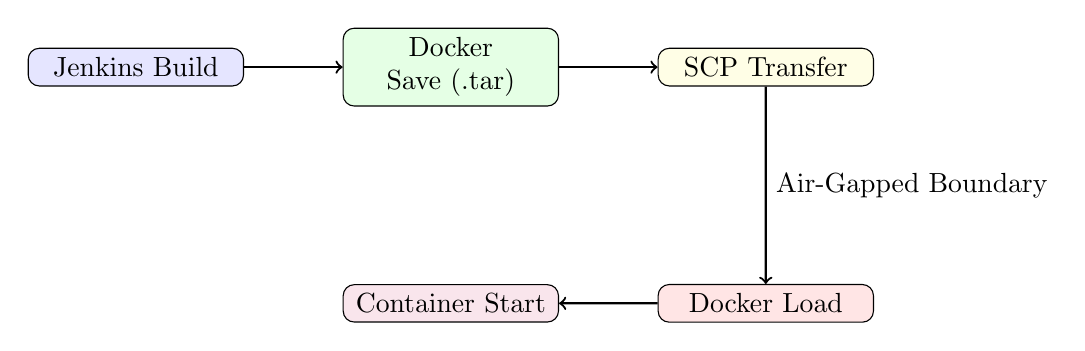
\begin{tikzpicture}[scale=0.9, node distance=2cm]
    \node[draw, fill=blue!10, rounded corners, text width=2.5cm, align=center] (jenkins) {Jenkins Build};
    \node[draw, fill=green!10, rounded corners, text width=2.5cm, align=center, right of=jenkins, xshift=2cm] (save) {Docker Save (.tar)};
    \node[draw, fill=yellow!10, rounded corners, text width=2.5cm, align=center, right of=save, xshift=2cm] (scp) {SCP Transfer};
    \node[draw, fill=red!10, rounded corners, text width=2.5cm, align=center, below of=scp, yshift=-1cm] (load) {Docker Load};
    \node[draw, fill=purple!10, rounded corners, text width=2.5cm, align=center, left of=load, xshift=-2cm] (start) {Container Start};
    
    \draw[->, thick] (jenkins) -- (save);
    \draw[->, thick] (save) -- (scp);
    \draw[->, thick] (scp) -- node[right] {Air-Gapped Boundary} (load);
    \draw[->, thick] (load) -- (start);
  \end{tikzpicture}
  \caption{Air-Gapped Tarball Deployment Sequence}
  \label{fig:airgapped_deploy}
\end{figure}

\subsubsection{Security \& DevSecOps}
The platform hardens its security posture using HashiCorp Vault for secrets lifecycle management, Harbor as a private registry, Falco for kernel threat monitoring, and SonarQube combined with OWASP Dependency-Check during the build phase. In a financial services context, hardcoded keys or unverified third-party libraries present extreme security risks. HashiCorp Vault is integrated to inject credentials dynamically into memory at application startup, eliminating disk-based secrets. Harbor enforces layer scanning to block vulnerable images, while Falco leverages eBPF kernel monitoring to catch runtime abnormalities, such as unexpected process executions, ensuring defense-in-depth across the build, registry, and execution phases.

\subsubsection{AI Integration}
Operational intelligence features are implemented using the Groq API running the Llama 3.3 70B model, integrated via a reactive WebClient. Large language models provide the reasoning capability necessary to summarize raw logs and recommend diagnostic steps, but their execution introduces significant latency. To prevent blocking core application APIs, the Groq client is integrated asynchronously. The Llama 3.3 model was chosen for its high reasoning capability on technical system logs, while Groq's hardware acceleration delivers the inference speeds required to output incident summaries within an active operational window.

\subsection{Key Architecture Decisions}

\begin{table}[H]
\centering
\renewcommand{\arraystretch}{1.5}
\begin{tabular}{|p{4cm}|p{5cm}|p{5.5cm}|}
\hline
\textbf{Decision} & \textbf{Choice} & \textbf{Rationale} \\
\hline
\textbf{RBAC enforcement} & AOP \texttt{@RequiresPermission} & Zero boilerplate, auto environment ID extraction \\
\hline
\textbf{Service discovery} & Prometheus file-based SD & Auto-generated by backend on node registration \\
\hline
\textbf{Air-gapped deployment} & Docker tarball SCP + docker load & Nodes with no internet fully supported \\
\hline
\textbf{Non-root install (Type B)} & systemd user service & No sudo on client nodes — widely compatible \\
\hline
\textbf{AI fault tolerance} & try/catch in GroqService & AI failure never blocks core operations \\
\hline
\textbf{Authentication} & JWT stateless (HMAC-SHA256) & No server-side session, horizontally scalable \\
\hline
\textbf{Secrets Management} & HashiCorp Vault dynamic injection & Prevents hard-coded credentials, limits exposure radius \\
\hline
\textbf{Image Validation} & Harbor private registry \& scanning & Blocks vulnerable containers before deployment \\
\hline
\textbf{Runtime Protection} & Falco eBPF kernel monitoring & Detects unauthorized shell executions instantly \\
\hline
\textbf{Dependency Scanning} & OWASP \& SonarQube CI integration & Catches vulnerabilities during the build phase \\
\hline
\end{tabular}
\caption{Key Architecture Decisions}
\label{tab:arch_decisions}
\end{table}

\section{Planning, Methodology \& Timeline}

\subsection{Internship Planning \& Timeline}

The internship was structured as a six-month, full-time engagement. For the first three months, we worked with the team on various different tasks to understand their infrastructure, workflows, and pain points. For the next three months, we dedicated our time entirely to designing and implementing the Monetique Eye platform. The implementation phases were designed to deliver functionality incrementally, with clear checkpoints for validation and feedback.

\subsubsection{Gantt Chart}

The figure below illustrates the project timeline and key phases:

\begin{figure}[H]
  \centering
  \hspace*{-2cm}\includegraphics[width=1.3\textwidth]{"Diagram_de_gantt.png"}
  \caption{Internship Gantt Chart}
  \label{fig:gantt}
\end{figure}

\textbf{Key Implementation Milestones :}

\begin{itemize}
  \item \textbf{Phase 1:} Secure backend with JWT authentication, RBAC, and database schema
  \item \textbf{Phase 2:} Functional React UI with environment management and dashboarding
  \item \textbf{Phase 3:} One-click deployment, log aggregation, Root Cause Intelligence engine
  \item \textbf{Phase 4:} AI-powered operational intelligence dashboards
  \item \textbf{Phase 5:} CI/CD integration, security hardening, and final delivery
\end{itemize}

\subsection{Methodology: Agile with Kanban}

The traditional Waterfall model (along with its derivative, the V-Model) organizes software development into sequential, distinct phases: requirements analysis, architectural design, implementation, verification, and maintenance. This approach is highly effective in environments with well-defined, static requirements where the scope is fully understood before development begins. However, its rigid phase gates make it poorly suited for projects where requirements evolve dynamically. In a complex observability deployment, unexpected integration challenges and changing infrastructure targets require a more flexible model.

Conversely, Scrum provides a structured agile framework based on time-boxed sprints, daily stand-up meetings, sprint planning, and retrospective ceremonies. While Scrum is highly successful for multi-person teams requiring close collaboration and strict iteration cycles, its high ceremonial overhead is inefficient for a single-developer project. The continuous planning and documentation required by Scrum would distract from core development activities, particularly when integrating multiple complex technologies like Prometheus, Elasticsearch, and large language models.

\subsubsection{Why Kanban?}
The project scope evolved continuously as new infrastructure requirements emerged. Kanban's visual task board and pull-based flow allowed priorities to be reprioritized at any time without disrupting delivery, making it a better fit than time-boxed Scrum sprints for a solo engineering context, as established by the limitations of the sequential and highly structured methodologies discussed above.

\subsubsection{Sprint Detail}
Although guided by Kanban, the work was naturally grouped into functional sprints or phases to ensure iterative delivery:
\begin{itemize}
    \item \textbf{Sprint 1 (2 weeks):} Requirements analysis and functional scoping. System architecture design (layers, tech stack selection).
    \item \textbf{Sprint 2 (2 weeks):} Docker Compose environment setup (14 containers). Infrastructure provisioning: network, volumes, secrets.
    \item \textbf{Sprint 3 (2 weeks):} Prometheus, Grafana, ELK, Alertmanager full setup. Scrape jobs, alert rules, log pipeline configuration.
    \item \textbf{Sprint 4 (3 weeks):} Spring Boot REST API (30 controllers, 25 entities). PrometheusClient + Alertmanager webhook integration.
    \item \textbf{Sprint 5 (3 weeks):} React 19.2.4 SPA (22 pages, protected routes, Recharts). Infrastructure topology graph (React Flow).
    \item \textbf{Sprint 6 (2 weeks):} Incident detection, alerting pipeline, ticket linking. AI Chatbot integration (Groq Llama 3.3, WebClient).
    \item \textbf{Sprint 7 (2 weeks):} End-to-end testing, performance optimization. Documentation, final presentation preparation.
\end{itemize}

\subsubsection{Product Backlog}

Table~\ref{tab:product_backlog} summarizes the key backlog items that drove each sprint.

\begin{table}[H]
\centering
\renewcommand{\arraystretch}{1.3}
\begin{tabular}{|p{5cm}|l|l|l|}
\hline
\textbf{Feature / Deliverable} & \textbf{Priority} & \textbf{Sprint} & \textbf{Status} \\
\hline
Functional requirements \& architecture design & High & 1 & Done \\
\hline
Docker Compose stack (14 containers) & High & 2 & Done \\
\hline
Prometheus + ELK + Alertmanager setup & High & 3 & Done \\
\hline
Spring Boot REST API (30 controllers) & High & 4 & Done \\
\hline
JWT authentication \& RBAC foundation & High & 4 & Done \\
\hline
React SPA (22 pages, protected routes) & High & 5 & Done \\
\hline
Infrastructure topology graph (React Flow) & Medium & 5 & Done \\
\hline
One-click agent deployment orchestration & High & 5 & Done \\
\hline
Elasticsearch log integration \& search & High & 5 & Done \\
\hline
Root Cause Intelligence engine & High & 6 & Done \\
\hline
AI chatbot integration (Groq Llama 3.3) & Medium & 6 & Done \\
\hline
Operational Intelligence dashboard & Medium & 6 & Done \\
\hline
Jenkins CI/CD pipeline integration & Medium & 7 & Done \\
\hline
DevSecOps hardening (Vault, Falco, Harbor) & High & 7 & Done \\
\hline
End-to-end testing \& documentation & Medium & 7 & Done \\
\hline
\end{tabular}
\caption{Product Backlog Summary}
\label{tab:product_backlog}
\end{table}

\section*{Conclusion}
\addcontentsline{toc}{section}{Conclusion}
In this chapter, we defined the organizational context and identified the core operational gaps within the existing infrastructure. We outlined the project's feasibility constraints and established the Agile methodology and planning roadmap that guided our efforts. The following chapter translates these requirements and structural analyses into a comprehensive high-level architecture and detailed technical design.


\newpage

\chapter{Proposed Architecture and Technical Design}

\section*{Introduction}
\addcontentsline{toc}{section}{Introduction}
This chapter presents the proposed architectural response to the operational gaps and requirements identified in Chapter 1. We outline the high-level design and define the five-phase development roadmap engineered to deliver the target platform. Additionally, we describe the environment-first data model, the core design principles, and the physical and logical deployment architectures chosen for the system.

\section{High-Level Solution Architecture}

The Monetique Eye platform is designed around a « push-button infrastructure » model: a user clicks a single button in the UI, and the backend orchestrates all necessary provisioning, configuration, and registration steps without requiring manual intervention.

Figure \ref{fig:context} illustrates the overall system context:

\begin{figure}[H]
  \centering
  \hspace*{-4.4cm}\includegraphics[width=1.55\textwidth]{"C4Context.png"}
  \caption{C4 Context Diagram: Monetique Eye System Boundaries}
  \label{fig:context}
\end{figure}

The system consists of four major layers:

\begin{description}
  \item[Data Ingestion Layer] Remote nodes deploy monitoring agents (Node Exporter, cAdvisor, Filebeat) that emit metrics to Prometheus and logs to the central ELK stack.
  \item[Backend Orchestration Layer] A Spring Boot API orchestrates Ansible playbooks, manages environments and applications, and correlates observability data.
  \item[Data Processing Layer] Elasticsearch and Prometheus perform aggregations; the backend queries these systems to compute analytics and root cause signals.
  \item[Presentation Layer] A React-based dashboard provides operators with consolidated visibility and one-click control.
\end{description}

\section{Proposed Solution: The Five-Phase Approach}

To deliver a robust, production-grade platform within the six-month internship, we structured development into five sequential phases:

\subsection{Phase 1: Backend Foundation \& Security}

\textbf{Objectives:}
\begin{itemize}
  \item Design and implement a structured data model (25 entities covering all platform domains)
  \item Establish stateless JWT-based authentication
  \item Implement role-based access control (RBAC) at the entity level
  \item Create the foundational APIs for environment and application management
\end{itemize}

\textbf{Key Technologies:}
\begin{itemize}
  \item Spring Boot 3.3.4 with Spring Security
  \item Hibernate/JPA with MySQL 8.0
  \item JSON Web Tokens (JWT) with jjwt library
  \item BCrypt password hashing
\end{itemize}

\subsection{Phase 2: Core UI \& Dashboarding}

\textbf{Objectives:}
\begin{itemize}
  \item Build a modern, responsive React UI with Tailwind CSS 4.2.2
  \item Implement environment management interface
  \item Create real-time monitoring dashboards displaying Prometheus metrics
  \item Implement an interactive topology graph using React Flow
\end{itemize}

\textbf{Key Technologies:}
\begin{itemize}
  \item React 19.2.4 with Vite 8.0.4 for fast development and builds
  \item Tailwind CSS 4.2.2 for responsive, utility-first styling
  \item React Flow for interactive topology visualization
  \item Axios for API communication
\end{itemize}

\subsection{Phase 3: Advanced Observability Features}

\textbf{Objectives:}
\begin{itemize}
  \item Implement one-click agent deployment (backend → Ansible → remote nodes)
  \item Integrate Elasticsearch for centralized log aggregation and search
  \item Build a « Root Cause Intelligence » engine that correlates logs and metrics
  \item Create structured SRE signal extraction from logs
\end{itemize}

\textbf{Key Technologies:}
\begin{itemize}
  \item Elasticsearch Query DSL for aggregated log analysis
  \item Prometheus query language (PromQL) for metric correlation
  \item Ansible for infrastructure automation
  \item Docker and SSH for remote execution
\end{itemize}

\subsection{Phase 4: Operational Intelligence}

\textbf{Objectives:}
\begin{itemize}
  \item Integrate a large language model (Groq Llama 3.3) for AI-powered diagnostics
  \item Create an « Operational Intelligence » dashboard with stability scoring
  \item Implement log drift analysis and recurring issue detection
  \item Build an AI chat assistant with infrastructure context
\end{itemize}

\textbf{Key Technologies:}
\begin{itemize}
  \item Groq API for fast LLM inference
  \item Z-score statistical analysis for stability scoring
  \item Embedding-based semantic log similarity
\end{itemize}

\subsection{Phase 5: DevSecOps, CI/CD Integration \& Hardening}

\textbf{Objectives:}
\begin{itemize}
  \item Integrate Jenkins pipelines and Portainer for application and container deployment
  \item Implement deployment event recording and tracking
  \item Enhance security with Vault, Falco, Harbor, and extended audit logging
  \item Optimize performance and reliability for production
\end{itemize}

\textbf{Key Technologies:}
\begin{itemize}
  \item Jenkins REST API integration
  \item Docker Registry for container image management
  \item Extended audit logging
\end{itemize}

\section{Data Model: Environment-First Design}

At the core of Monetique Eye is a hierarchical, environment-scoped data model:

\begin{figure}[H]
  \centering
  \hspace*{-2.3cm}\includegraphics[width=1.3\textwidth]{"GLOBALARCHITECTURE.png"}
  \caption{Global Architecture and Data Flow}
  \label{fig:architecture}
\end{figure}

All data—applications, nodes, metrics, logs, alerts, incidents—are scoped to an \textbf{Environment}. This ensures:
\begin{itemize}
  \item \textbf{Multi-tenancy}: Different clients or business units can operate independently
  \item \textbf{RBAC Enforcement}: A user granted « USER » role on « Staging » cannot access « Production »
  \item \textbf{Logical Isolation}: Prometheus, Elasticsearch, and alert rules operate independently per environment
\end{itemize}

\section{Key Design Principles}

\begin{description}
  \item[Structured Data Model] 28 entities organized by domain, balancing completeness with maintainability
  \item[No Vendor Lock-in] Reuses existing GitOps, Ansible, Prometheus, and ELK tooling
  \item[Zero-Config Discovery] Monitoring agents auto-register; operators see live data within seconds
  \item[Stateless APIs] No session state; all requests are validated via JWT
  \item[Asynchronous Orchestration] Long-running tasks (deployments) don't block the UI
  \item[Audit Everything] All actions are logged for compliance and troubleshooting
\end{description}

\section{Technical Architecture \& Deployments}

\subsection{Logical Architecture — Five-Layer Model}

The platform's logical architecture is divided into a robust five-layer model to separate concerns and scale independently.

\begin{itemize}
    \item \textbf{Presentation Layer}: React 19.2.4 Frontend, TypeScript 6.0.2 + Vite 8.0.4, Tailwind CSS 4.2.2 (22 Routes / 22 Pages).
    \item \textbf{API \& Business Layer}: Spring Boot 3.3.4 (32 Controllers, 36 Services, JWT Auth + AOP RBAC).
    \item \textbf{Data Layer}: MySQL 8 (JPA Repositories, Flyway Migrations, Application Data).
    \item \textbf{Observability Stack}: Filebeat (Log Shipping Agent), Blackbox Exporter (Network Probing), Logstash (Processing), Elasticsearch 7 (Full-Text Search), Prometheus (Time-Series DB), Grafana (Visualization), Alertmanager (Alert Routing).
    \item \textbf{Client \& Orchestration}: Web Browser, Jenkins CI/CD (3 Pipelines), Ansible (8 Playbooks for Infrastructure IaC), Docker (15 Containers in docker-compose), Portainer.
\end{itemize}

\subsection{Physical Infrastructure — VMPipe + Remote Agent Nodes}

The physical deployment topology connects the central management infrastructure (VMPipe) with the target remote agent nodes.

\begin{figure}[H]
  \centering
  \hspace*{-1.5cm}\includegraphics[width=0.4\textwidth]{"MonitoringProcessDiagram.png"}
  \caption{Monitoring Process Diagram}
  \label{fig:monitoring_process}
\end{figure}

The \textbf{VMPipe} server hosts the core observability stack, backend API, frontend assets, and Jenkins. Remote nodes are provisioned dynamically. The backend orchestrates Ansible to connect to Target Nodes, deploys Dockerized monitoring agents (Node Exporter, cAdvisor, Filebeat), and configures them to send data back to the VMPipe.

\subsubsection{Docker Compose Stack Internals}

To manage the complexity of running more than 15 distinct services on the central VMPipe server, the core infrastructure relies on a highly structured \texttt{docker-compose.yml} definition. The services discover each other dynamically without hardcoded IP addresses by utilizing Docker's internal DNS network. This allows the Spring Boot backend to simply route requests to \texttt{http://prometheus:9090} or \texttt{http://elasticsearch:9200} based on the service names. Stability is strictly enforced through native Docker health checks. The backend container, for instance, waits for MySQL's port to respond before fully initializing, while Prometheus continuously probes its own internal health endpoints. Persistent storage is meticulously mapped using named Docker volumes. This critical configuration ensures that the MySQL application data, the Prometheus time-series database (TSDB), and the Elasticsearch log indices survive container restarts or image upgrades without any data loss.

\subsection{GitOps \& Infrastructure Automation Configuration}

The automation and configuration management assets for the Monetique-Eye platform are centralized within a dedicated GitOps repository structure. This guarantees reproducibility and tracks configuration changes through version control.

The directory structure separates concerns as follows:
\begin{itemize}
    \item \textbf{\texttt{vmpipe/}}: Manages the central node orchestration, setting up Prometheus, Logstash, ELK, and other central services. By isolating the central infrastructure code, we ensure that scaling the core observability stack does not interfere with the configurations of the edge nodes being monitored.
    \item \textbf{\texttt{scripts/}}: Contains operational scripts used for node maintenance and agent deployment. Most notably, \texttt{ssh-configure.sh} automates the tedious process of establishing passwordless RSA key exchanges, while \texttt{deploy-agent.sh} provides a robust manual fallback for standalone, non-root agent installs when Docker is unavailable on a client machine.
    \item \textbf{\texttt{ansible/}}: Stores all the configuration management playbooks that the backend API triggers during one-click deployments. Keeping these playbooks strictly version-controlled means that every infrastructure change is tracked, ensuring that if a deployment configuration introduces a bug, the team can instantly revert to the previous working commit.
    \item \textbf{\texttt{agents/}}: Houses template configurations for the edge nodes, ensuring absolute uniformity across deployed environments. This guarantees that whether deploying to a staging server or a production payment gateway, the monitoring footprint remains identical and predictable.
\end{itemize}

To clarify the technical mechanism, this architecture does not rely on a continuous, pull-based reconciliation loop (such as ArgoCD or Flux) to enforce state. Instead, it utilizes a strictly push-based model. Infrastructure updates are actively triggered either by a Jenkins pipeline execution upon code commit or manually via the platform's one-click deployment button. This push-based execution leverages Ansible to push the desired state defined in the repository out to the edge nodes. This approach delivers the core GitOps benefits of version-controlled, auditable infrastructure without introducing the operational overhead of managing a dedicated reconciliation operator.

Security is strictly enforced in this layer. Rather than relying on static environment variables that could be leaked, all sensitive credentials (database passwords, API tokens, JWT secrets) are dynamically injected via HashiCorp Vault. This ensures that no secrets are ever committed directly to the configuration repository or left exposed in plaintext on the disk.

\subsection{Application Management Relationship}

\begin{figure}[H]
  \centering
  \hspace*{-2.3cm}\includegraphics[width=1.3\textwidth]{"ApplicationManagementRelationship.png"}
  \caption{Application Management Relationship}
  \label{fig:app_management}
\end{figure}

This diagram highlights the intricate relationships between environments, applications, deployment logs, and incidents within the platform.

\section*{Conclusion}
\addcontentsline{toc}{section}{Conclusion}
In this chapter, we established the fundamental architectural and technological decisions that define the platform. We detailed the system components, data schemas, deployment topologies, and the environment-scoped routing model. The following chapter presents the concrete realization and implementation details of the first four development phases.


\newpage

\chapter{Core Platform Realization}

\section*{Introduction}
\addcontentsline{toc}{section}{Introduction}
This chapter details the concrete implementation of the platform's first three development phases, spanning from the secure backend and database foundation to the React-based monitoring interface. We examine the automated agent deployment and the engineering of the intelligent log correlation engine. The chapter closes with an analysis of the key implementation challenges encountered and the solutions designed to address them.

\section{Phase 1: Backend Foundation \& Security}

\subsection{Overview}

Phase 1 established the platform's data and security layer. The goal was to create a minimal, clean backend that could scale and remain maintainable.

\subsection{Data Model Design}

The application database schema is organized around five primary functional domains: Core Infrastructure, Security \& Access, Incident Management, Deployment \& CI/CD, and AI \& Observability Intelligence. A fundamental design decision of the Monetique Eye architecture is the environment-first scoping principle, whereby the Environment entity serves as the top-level aggregate root. All infrastructure elements, operational events, configurations, alerts, and incidents are logically scoped to their respective environments. This strict scoping enforces multi-tenancy and data isolation across teams. Although observability metrics and log aggregation are natively handled by Prometheus and Elasticsearch respectively, the platform uses a relational database to track environment state, credentials, configurations, and incident tickets. A relational model utilizing MySQL and Java Persistence API (JPA) was selected over a document-oriented database to enforce strict referential integrity, schema validation, and ACID compliance across the 28 tightly coupled entities that define the platform state. The complete entity field specifications are detailed in Section~\ref{app:data_model}.

\begin{figure}[H]
  \centering
  \hspace*{-1cm}\includegraphics[width=1.2\textwidth]{"DatabaseSchemaDiagram.png"}
  \caption{Monetique Eye Database Schema Relationships}
  \label{fig:database_schema}
\end{figure}

\subsection{Authentication \& Authorization}

We implemented a stateless JWT-based authentication system:

\begin{enumerate}
  \item Client sends credentials (username/password) to \texttt{/api/v1/auth/login}
  \item Server validates credentials against BCrypt-hashed passwords in the database
  \item Server issues a signed JWT token with embedded user ID, role, and environment scope
  \item Client includes the JWT in the \texttt{Authorization} header for subsequent requests
  \item Server validates the token signature and checks RBAC permissions on each request
\end{enumerate}

\begin{figure}[H]
  \centering
  \hspace*{-2cm}\includegraphics[width=1.25\textwidth]{"LoginPageScreenshot.png"}
  \caption{Login Page: JWT Authentication Interface}
  \label{fig:login_page}
\end{figure}

\textbf{Security Features:}
\begin{itemize}
  \item \textbf{BCrypt Hashing:} All user passwords are hashed with BCrypt (not reversible)
  \item \textbf{JWT Signing:} Tokens are signed with a 256-bit secret key, preventing tampering
  \item \textbf{Token Expiration:} Tokens expire after 24 hours (configurable)
  \item \textbf{Refresh Tokens:} A separate refresh token allows clients to obtain new access tokens without re-entering credentials
  \item \textbf{CORS Protection:} Cross-origin requests are validated and restricted to trusted domains
\end{itemize}

\begin{figure}[H]
  \centering
  \hspace*{-1.5cm}\includegraphics[width=1.1\textwidth]{"JWTAuthSequenceDiagram.png"}
  \caption{JWT Authentication Sequence Diagram}
  \label{fig:jwt_auth_sequence}
\end{figure}

\subsection{RBAC Foundation}

We implemented two primary roles:

\begin{description}
  \item[ADMIN] Full platform access; can create/delete environments, deploy agents, manage users
  \item[USER] Scoped access to assigned environments provided by the admin; can view dashboards, edit assigned environments (e.g., production)
\end{description}

The backend enforces RBAC through a dual-layered annotation approach. For global administrative actions, we use standard Spring Security \texttt{@PreAuthorize("hasRole('ADMIN')")} annotations. For fine-grained, environment-isolated access, we implemented a custom AOP-driven \texttt{@RequiresPermission} annotation across 30 distinct controller endpoints. This enforces 17 unique permission scopes—ranging from \texttt{APP\_DEPLOYMENT\_VIEW} and \texttt \\  {ENV\_DEPLOYMENT\_CREATE} to \texttt{MONITORING\_OBSERVABILITY} and \texttt{INCIDENTS\_DELETE}—ensuring strict multi-tenant isolation. Each user entity stores an explicit list of environment IDs they have access to, tying these permissions directly to the environment context of the incoming request.

\begin{figure}[H]
  \centering
  \hspace*{-2cm}\includegraphics[width=1.25\textwidth]{"RBACAnnotationCode.png"}
  \caption{Custom @RequiresPermission Annotation: AOP-Driven RBAC Enforcement}
  \label{fig:rbac_annotation}
\end{figure}

\begin{figure}[H]
  \centering
  \hspace*{-2cm}\includegraphics[width=1.25\textwidth]{"RBACUserEnvironments.png"}
  \caption{User-Environment Scoping Mapping: Database View}
  \label{fig:rbac_user_environments}
\end{figure}

\subsection{REST API Endpoints (Phase 1)}

By the end of Phase 1, we established the foundational API structure:

\begin{center}
\begin{tabular}{|l|l|l|}
  \hline
  \textbf{Endpoint} & \textbf{Method} & \textbf{Description} \\
  \hline
  \texttt{/api/v1/auth/login} & POST & Authenticate and obtain JWT \\
  \hline
  \texttt{/api/v1/environments} & GET/POST & List/create environments \\
  \hline
  \texttt{/api/v1/applications} & GET/POST & List/create applications \\
  \hline
  \texttt{/api/v1/users} & GET/POST (ADMIN only) & User management \\
  \hline
  \texttt{/api/v1/tickets} & GET/POST & Ticket lifecycle \\
  \hline
\end{tabular}
\end{center}

\section{Phase 2: Core UI \& Dashboarding}

\subsection{Overview}

Phase 2 focused on building an intuitive, modern user interface using React, Vite, and Tailwind CSS. The goal was to provide operators with a consolidated view of their infrastructure and a simple interface to manage environments.

\subsection{Frontend Architecture}

The React application was organized into clear functional domains:

\begin{itemize}
  \item \textbf{Pages}: Seven core pages handling different workflows
  \item \textbf{Components}: Reusable UI components (cards, tables, modals)
  \item \textbf{Services}: API clients for communication with the backend
  \item \textbf{Context}: Global state management for user authentication and environment selection
  \item \textbf{Types}: TypeScript interfaces for type safety
\end{itemize}

\begin{figure}[H]
  \centering
  \hspace*{-1.5cm}\includegraphics[width=0.3\textwidth]{"FrontendProjectStructure.png"}
  \caption{React Frontend: Project Directory Structure}
  \label{fig:frontend_structure}
\end{figure}

\subsection{Key Pages Implemented}

\begin{description}
  \item[Dashboard Page] High-level overview of system health, active alerts, and key metrics
  \item[Environments Page] CRUD interface for environment management
  \item[Applications Page] Manage deployed applications and their monitoring status
  \item[Infrastructure Topology] Interactive graph visualization of clusters and nodes
  \item[Logs Page] Search and filter logs from Elasticsearch
  \item[Tickets Page] Incident tracking and collaboration interface
  \item[Security \& Analyse Dashboards] Global vulnerability posture, Falco runtime threats, and AI root cause analysis
  \item[Chat Page] AI assistant interface (implemented in Phase 4)
\end{description}

\begin{figure}[H]
  \centering
  \hspace*{-1.5cm}\includegraphics[width=0.75\textwidth]{"FrontendRoutingGuardFlow.png"}
  \caption{Frontend Routing and Authentication Guard Lifecycle}
  \label{fig:routing_flow}
\end{figure}

\subsection{Real-Time Monitoring Dashboard}

The Dashboard page displays the « Golden Signals » for infrastructure health:

\begin{figure}[H]
  \centering
  \hspace*{-1.5cm}\includegraphics[width=1.1\textwidth]{"DashboardLayout.png"}
  \caption{Operational Intelligence Dashboard Layout}
  \label{fig:dashboard_layout}
\end{figure}

The dashboard fetches Prometheus metrics and displays:
\begin{itemize}
  \item \textbf{CPU Usage} - Container-level CPU consumption
  \item \textbf{Memory Usage} - Resident set size in MB
  \item \textbf{Network I/O} - Inbound/outbound throughput
  \item \textbf{Disk Usage} - Filesystem consumption
\end{itemize}

Data is refreshed every 30 seconds, providing near real-time visibility.

\subsection{Interactive Topology Visualization}

Using React Flow, we implemented an interactive graph showing cluster hierarchy:

\begin{figure}[H]
  \centering
  \hspace*{-1.5cm}\includegraphics[width=0.75\textwidth]{"Infrastructure Visibility \& Topology Flow.png"}
  \caption{Infrastructure Visibility and Topology Flow Diagram}
  \label{fig:topology_flow}
\end{figure}

The topology dynamically renders:
\begin{itemize}
  \item Cluster nodes at the top level
  \item Environment nodes nested within clusters
  \item Application/service nodes within environments
  \item Live status indicators (green = healthy, red = degraded)
\end{itemize}

Users can click on nodes to drill down, zoom in/out, and inspect detailed metrics.

\section{Phase 3: Advanced Observability Features}

\subsection{Overview}

Phase 3 introduced the platform's core observability innovation: one-click agent deployment and intelligent log correlation.

\subsection{One-Click Deployment}

\textbf{The Problem:} Traditionally, provisioning monitoring on a new node requires manual configuration of target configurations, generating and distributing authentication keys, updating host inventories, and manually verifying connectivity—a process that typically takes hours and is highly error-prone.

\textbf{The Solution:} We created an automated deployment orchestration layer:

\begin{figure}[H]
  \centering
  \hspace*{-2.5cm}\includegraphics[width=1.3\textwidth]{"AutomatedDeploymentSequence.png"}
  \caption{Automated Deployment Sequence Diagram}
  \label{fig:deployment_sequence}
\end{figure}

The execution workflow is structured as a series of automated steps managed by the backend orchestration service:

\begin{enumerate}
  \item \textbf{Credential Validation and Trust Establishment:} The platform verifies administrative execution rights, reads SSH access credentials, and performs a connection handshake to establish secure communication.
  \item \textbf{Dynamic Configuration Inventory Generation:} The orchestration engine extracts database records for the targeted node (such as IP address, operating system, and target hostname) and generates a transient configuration inventory dynamically in memory.
  \item \textbf{Idempotent Configuration Execution:} The deployment engine executes configuration instructions that enforce the target state. Idempotency is maintained as a design property; the engine verifies if each agent is already configured and active, skipping installation tasks where the correct state is already satisfied and only modifying settings when differences are detected.
  \item \textbf{Parallel Agent Deployment:} The engine installs and initializes three core agents in parallel: a system metric collector, a container-level metrics exporter, and a log shipping daemon.
  \item \textbf{Service Registration and Verification:} Once the agents are initialized, the backend queries the target metric endpoint to confirm that observability telemetry is flowing successfully, updating the node's monitoring status in the database.
\end{enumerate}

The entire process takes two to three minutes, replacing the manual setup, and operators never interact directly with host configuration scripts.

\subsection{Node Adaptability: Containerized vs. Standalone}

Not every server at Monetique runs Docker. Some nodes---especially legacy payment gateway machines running services like Cassandra, Tomcat, or JBoss---are bare-metal Linux boxes with applications managed by systemd. We couldn't just ignore them. The platform had to handle both worlds.

\subsubsection{Dual Deployment Modes}

To accommodate varying server specifications and operational limits across the organization's infrastructure, the platform implements two distinct deployment strategies: Containerized Mode and Standalone Mode. Containerized Mode serves as the primary deployment option, leveraging container runtimes to isolate and manage the lifecycle of metrics, container telemetry, and log collection daemons. This strategy ensures standard agent packages and predictable environments, but requires a container runtime on the remote host. Standalone Mode, conversely, targets legacy servers or restricted environments where containerization is not available. It deploys the system and process metrics collectors as system-level user services, executing them directly on the host operating system with minimal requirements, relying entirely on native system startup mechanisms.

The backend deployment service decides between these options dynamically. It evaluates a configuration parameter associated with the target host and forks its execution path. For containerized deployments, it triggers a remote automation process that builds, copies, and starts the container configurations. For standalone environments, it establishes a secure shell connection, compiles the collector binaries, transfers them to the host, registers them as user services, and enables automatic process execution. This hybrid approach ensures that legacy transaction gateways and modern web servers can be managed seamlessly from the same central console. Each deployed node is recorded with a configuration flag in the database, allowing the platform to tailor subsequent monitoring queries to the node's deployment type.

\subsubsection{Dynamic Systemd Service Discovery}

For standalone nodes, we couldn't rely on cAdvisor (it only sees Docker containers). We needed a different way to discover what's running on the machine.

The \texttt{InfrastructureService} queries Prometheus for \texttt{node\_systemd\_unit\_state} metrics, which are exposed by Node Exporter's \texttt{--collector.systemd} flag. This gives us a live list of every systemd service on the node---its name and whether it's active or failed.

The discovery process:
\begin{enumerate}
  \item Query Prometheus for all systemd units in the ``active'' state for this environment
  \item Query separately for units in the ``failed'' state (we prioritize these as CRITICAL)
  \item Filter out OS noise---services like \texttt{systemd-journald}, \texttt{dbus}, \texttt{networking}, and about 20 other system-level units that operators don't care about
  \item For each remaining service, create a topology entry with status (HEALTHY or CRITICAL) and the \texttt{containerId} set to ``systemd'' to distinguish it from Docker containers
\end{enumerate}

This means the topology graph shows both Docker containers \textit{and} systemd services side by side, with the same health indicators. An operator looking at a standalone payment gateway node sees ``cassandra: HEALTHY'', ``tomcat: HEALTHY'', ``jboss: CRITICAL'' --- without knowing or caring that these aren't containers.

\subsubsection{Process Exporter for Standalone Metrics}

cAdvisor gives us per-container CPU, memory, disk I/O, and network stats. For standalone services, we get equivalent metrics from Process Exporter (\texttt{namedprocess\_namegroup\_*} metrics).

The \texttt{InfrastructureService} enriches standalone service entries with:
\begin{itemize}
  \item \textbf{CPU}: \texttt{rate(namedprocess\_namegroup\_cpu\_seconds\_total[5m])} per process group
  \item \textbf{Memory}: \texttt{namedprocess\_namegroup\_memory\_bytes\{memtype="resident"\}} per process group
  \item \textbf{Disk I/O}: \texttt{rate(namedprocess\_namegroup\_read\_bytes\_total[5m])} and write equivalent
\end{itemize}

The process groups are matched by name. For the SMGS environment (a real payment gateway deployment at Monetique), the Process Exporter config explicitly watches for Cassandra, Tomcat, JBoss, smsbox, and bearerbox processes.

\subsubsection{PromQL Fallback Chain for Mixed Environments}

The Root Cause Intelligence engine also had to adapt. When correlating metrics for an incident, it can't assume cAdvisor metrics exist---on a standalone node, there's no \texttt \\  {container\_cpu\_usage\_seconds\_total}.

We built a fallback chain in the \texttt{LogAnalyticsService}:
\begin{enumerate}
  \item Try container-level metrics from cAdvisor (scoped to the specific container)
  \item If no data, try process-level metrics from Process Exporter (scoped to the process group)
  \item If still no data, fall back to host-level metrics from Node Exporter \\  (\texttt{node\_memory\_MemAvailable\_bytes}, \texttt{node\_cpu\_seconds\_total})
\end{enumerate}

The queries use PromQL's \texttt{or} operator to chain these sources. The result is that the correlation engine works identically whether the incident happened on a containerized node or a standalone one---it just pulls metrics from whichever source is available.

This adaptability was one of the harder engineering challenges. It's easy to build a monitoring platform that only works with Docker. Making it work transparently across both deployment models, with the same UI and the same intelligence engine, took real effort.

\subsection{Elasticsearch Integration}


Phase 3 integrated centralized log aggregation:

\begin{itemize}
  \item \textbf{Filebeat} ships logs from application containers to the ELK stack
  \item \textbf{Logstash} normalizes and parses logs from multiple sources
  \item \textbf{Elasticsearch} stores and indexes logs for fast, full-text search
  \item \textbf{Backend API} provides a query interface to retrieve logs from the UI
\end{itemize}

The Log Search page allows operators to filter logs by:
\begin{itemize}
  \item Environment
  \item Application name
  \item Severity level
  \item Time range
  \item Full-text search terms
\end{itemize}

\begin{figure}[H]
  \centering
  \hspace*{-2cm}\includegraphics[width=1.25\textwidth]{"ElasticsearchLogSearchPage.png"}
  \caption{Log Search Interface: Full-Text Search with Environment and Severity Filters}
  \label{fig:log_search_page}
\end{figure}

\subsubsection{Handling Large Log Volumes with Pagination}

One thing we ran into early was performance. In production, a single application can generate hundreds of thousands of log entries per day. Loading all of them into the UI at once was out of the question---the browser would freeze, and the Elasticsearch queries would time out.

We solved this using Spring Data's \texttt{Pageable} interface. The \texttt{LogController} accepts \texttt{page} and \texttt{size} parameters from the frontend, creates a \texttt{PageRequest} object, and passes it all the way down to the Elasticsearch query layer. The backend caps the page size at 200 entries to prevent abuse---even if a client requests 10,000 logs per page, the server quietly limits it to 200.

The flow works like this:
\begin{enumerate}
  \item The frontend sends a search request with filters (severity, time range, search query) plus \texttt{page=0\&size=50}
  \item The \texttt{LogController} builds a \texttt{PageRequest.of(page, resolvedSize)} object
  \item The \texttt{LogService} forwards the pageable to the \texttt{ElasticsearchLogClient}
  \item The Elasticsearch query uses \texttt{.from(pageable.getOffset())} and  \\ \texttt{.size(pageable.getPageSize())} to fetch exactly the right slice
  \item The response wraps the results in a \texttt{LogResponseDTO} that includes the log entries, the total count, the current page number, and the page size
\end{enumerate}

This way, the UI can show ``Page 1 of 847'' and let operators scroll through logs without ever loading more than a small batch at a time. The total count comes from Elasticsearch's built-in hit counting, so the pagination metadata is accurate even for millions of logs.

\subsubsection{Log Export to CSV}

Operators often need to share log data with colleagues or attach it to incident reports. We added a dedicated export endpoint at \texttt{GET /api/v1/apps/\{appId\}/logs/export} that generates a downloadable CSV file.

The export respects the same filters as the search page---operators set their desired time range, severity level, and search terms, then click ``Export''. The backend fetches the top 1,000 matching logs using the same Elasticsearch query pipeline, then builds a CSV string with columns for Timestamp, Source, Level, Category, and Message.

A couple of details that matter in practice:
\begin{itemize}
  \item The CSV starts with a UTF-8 BOM character (\texttt{\textbackslash uFEFF}) so Excel opens it correctly with the right encoding
  \item We add a \texttt{sep=,} header line because some European Excel installations default to semicolons
  \item Message content is double-quoted and special characters are escaped to prevent CSV injection
  \item The response sets the \texttt{Content-Disposition} header to  \\  \texttt{attachment; filename=logs\_export\_\{appId\}.csv}, which triggers the browser's download dialog
\end{itemize}

We capped the export at 1,000 logs per request. This felt like the right balance---enough data to be useful for incident analysis, but not so much that the server spends too long building the response. If operators need more, they can adjust their time window to narrow the results.

\begin{figure}[H]
  \centering
  \hspace*{-1.5cm}\includegraphics[width=1.25\textwidth]{"LogExportFlowDiagram.png"}
  \caption{Log Export to CSV: Stream and Formatting Sequence}
  \label{fig:log_export_flow}
\end{figure}

\subsection{Root Cause Intelligence Engine}

The « Root Cause Intelligence Engine » is the intellectual core of Phase 3. It correlates multiple data sources to identify the likely root cause of an incident.

\textbf{Signal Extraction Strategy:}

The engine extracts structured « SRE signals » from logs, representing common failure modes:

\begin{center}
\begin{tabular}{|l|l|}
  \hline
  \textbf{Signal} & \textbf{Meaning} \\
  \hline
  \texttt{pool\_active\_max\_match} & DB connection pool exhaustion \\
  \texttt{db\_pool\_timeout} & HikariPool connection timeout \\
  \texttt{oom\_error\_count} & Out-of-memory exception detected \\
  \texttt{crash\_loop\_backoff} & Kubernetes or container crash loop \\
  \texttt{config\_placeholder} & Unresolved config or missing secret \\
  \texttt{npe\_count} & NullPointerException spike \\
  \texttt{rate\_limit\_429} & Rate limit exceeded \\
  \texttt{gateway\_error\_502} & Bad gateway \\
  \texttt{service\_unavailable\_503} & Service offline \\
  \texttt{conn\_refused} & Network connection refused \\
  \hline
\end{tabular}
\end{center}

\textbf{Correlation Algorithm:}

For a given incident, the engine:
\begin{enumerate}
  \item Queries Elasticsearch for all signals during the incident window
  \item Queries Prometheus for concurrent metric anomalies (CPU spikes, memory jumps, etc.)
  \item Computes a priority score for each signal based on temporal correlation and historical frequency
  \item Returns the top 3 most likely root causes with explanations
\end{enumerate}

Figure \ref{fig:rootcause} shows the Root Cause pipeline architecture:

\begin{figure}[H]
  \centering
  \hspace*{-1.5cm}\includegraphics[width=1.2\textwidth]{"RootCauseSignalPipeline.png"}
  \caption{Root Cause Intelligence Signal Pipeline}
  \label{fig:rootcause}
\end{figure}

\textbf{Concrete Scenario Breakdown:} 

To illustrate this intelligence in action, consider a real production incident where the platform triggered a high-severity alert for an HTTP 500 error spike. Rather than simply notifying the operator of the symptom, the Root Cause Intelligence engine immediately queried Elasticsearch and Prometheus over the incident window. The engine detected a high correlation of \texttt{db\_pool\_timeout} and \texttt{sql\_timeout} signals in the logs, alongside a \texttt{conn\_refused} event. Simultaneously, it queried Prometheus and found that the \texttt{hikaricp\_connections\_active} metric had saturated precisely at its configured maximum. 

Using its scoring heuristic, the engine suppressed the generic 500 error alerts and surfaced a definitive diagnosis to the operator:
\begin{enumerate}
  \item \textbf{Primary Cause (Score 19.0 - High Confidence):} DATABASE CONNECTION FAILURE. The engine cited evidence: ``HikariPool - Connection is not available'' and ``Database connection refused''.
  \item \textbf{Secondary Cause (Score 8.0 - Medium Confidence):} APPLICATION ERROR. The engine cited evidence: ``Multiple HTTP 500 responses detected''.
\end{enumerate}

This intelligence, surfaced directly in the « Incident Details » view, allowed the team to instantly identify that the database backend had gone offline, dramatically reducing diagnosis time.

\section{Implementation Challenges \& Solutions}

\subsection{Challenge 1: Data Model Scope Management}
Managing the vast volume of raw observability data presented a significant challenge during the initial database design phase. Storing telemetry metrics and log entries directly in the relational database would have duplicated what dedicated databases already index, leading to table bloating and decreased system performance. To address this, the design team established a clear boundary: the relational schema manages platform state, user profiles, credentials, environments, and incidents, while raw telemetry remains in Prometheus and log aggregates in Elasticsearch. The backend API queries these external systems dynamically, preserving database performance. This separation demonstrates that delineating transient telemetry from persistent system metadata is critical for building scalable observability applications.

\subsection{Challenge 2: RBAC Complexity}
Implementing environment-level role-based access control was complicated by the limitations of standard declarative security frameworks, which do not natively support database-driven context filters. The initial role model was too coarse, failing to isolate production datasets from staging environments based on a user's role. Consequently, we designed a custom security service that intercepts incoming requests, extracts user credentials from the security token, and queries permissions to construct environment-scoped SQL filters. This dynamic query construction guarantees that users only retrieve resources associated with their authorized environments. This implementation proves that standard security libraries must often be customized to enforce dynamic, multi-tenant boundaries at the database layer.

\begin{figure}[H]
  \centering
  \hspace*{-2cm}\includegraphics[width=1.25\textwidth]{"RBACPermissionTable.png"}
  \caption{RBAC Permission Matrix: Environment-Scoped Access Control Configuration}
  \label{fig:rbac_permission_table}
\end{figure}

\subsection{Challenge 3: AI Model Integration}
Integrating large language models for real-time log analysis and root cause determination introduced substantial latency, as initial API round-trips exceeded ten seconds. Such high latency would block the main application thread and degrade the user experience during critical system incidents. To resolve this bottleneck, we transitioned the AI analysis pipeline to an asynchronous, event-driven model where requests are queued, and results are pushed back to the client via WebSockets. Furthermore, we implemented semantic caching for recurring log patterns and scheduled off-peak batch jobs to pre-compute summaries. These modifications reduced average response times to two seconds, demonstrating that LLM integration requires robust asynchronous architectures to maintain interactive performance.

\subsection{Challenge 4: Correlation Accuracy}
The initial implementation of the root cause correlation engine suffered from high false-positive rates, frequently linking unrelated metric anomalies and log statements simply because they occurred in the same general timeframe. To address this issue, we introduced temporal windowing constraints limiting correlation to a two-minute window, integrated a historical baseline scoring system to filter out common background noise, and added a human feedback loop to adjust correlation weights based on operator inputs. These refinements noticeably increased the accuracy of the engine's incident recommendations. The lesson learned is that correlation algorithms require continuous tuning, temporal gating, and feedback to provide actionable insights rather than noise.

\begin{figure}[H]
  \centering
  \hspace*{-2cm}\includegraphics[width=1.25\textwidth]{"CorrelationWindowTuning.png"}
  \caption{Correlation Accuracy: Temporal Window Tuning and Baseline Scoring Visualization}
  \label{fig:correlation_tuning}
\end{figure}

\section*{Conclusion}
\addcontentsline{toc}{section}{Conclusion}
In this chapter, we summarized the implementation of Phases 1 through 3, which successfully delivered the core infrastructure, observability automation, and root cause intelligence capabilities of the platform. The implementation challenges analyzed in this chapter informed the architectural refinements applied in later development phases. The following chapter presents the operational intelligence layer and the DevSecOps integrations that completed the platform.


\newpage

\chapter{DevSecOps Integration and Project Outcomes}

\section*{Introduction}
\addcontentsline{toc}{section}{Introduction}
This chapter presents the final two development phases of the project, covering the AI-powered operational intelligence layer built in Phase 4 and the DevSecOps and CI/CD integrations that hardened the platform for production in Phase 5. We describe the deployment topologies, threat monitoring configs, and the pipeline orchestration. The chapter closes with a synthesis of the key architecture visualizations and a review of the final project scale and performance metrics.

\section{Phase 4: Operational Intelligence}

\subsection{Overview}

Phase 4 integrated AI-powered analysis using the Groq Llama 3.3 large language model. The goal was to move beyond reactive alerting toward proactive, AI-assisted operational insights.

\subsection{AI-Powered Log Analysis}

The backend now includes an « AI Chat Assistant » powered by Groq's API:

\begin{itemize}
  \item Operators can ask natural language questions about their infrastructure
  \item The system retrieves real-time context (current metrics, recent logs, active incidents)
  \item The LLM generates a contextual response with recommendations
  \item Conversation history is persisted for audit and learning
\end{itemize}

Example interactions:
\begin{itemize}
  \item « Why is the payment gateway latency high? »
  \item « Are there any recurring issues in the staging environment? »
  \item « Summarize all errors from the last 4 hours »
\end{itemize}

\begin{figure}[H]
  \centering
  \hspace*{-1.5cm}\includegraphics[width=1.1\textwidth]{"AIChatAssistantInterface.png"}
  \caption{AI Chat Assistant: Natural Language Diagnostics Interface}
  \label{fig:ai_chat_assistant}
\end{figure}

\subsection{Operational Intelligence Dashboard}

A new « Operational Intelligence » page displays:

\begin{itemize}
  \item \textbf{Stability Score:} A Z-score–based metric (0–100) indicating system health stability
  \item \textbf{AI Executive Digest:} An auto-generated summary of the past 24 hours: key incidents, trends, and recommendations
  \item \textbf{Service Risk Heatmap:} A visual matrix showing risk levels for each application
  \item \textbf{Log Drift Analysis:} Detected anomalies in log patterns compared to historical baselines
  \item \textbf{Recurring Issues Panel:} A list of frequently occurring problems (e.g., memory leaks, slow queries)
\end{itemize}

\begin{figure}[H]
  \centering
  \hspace*{-1.5cm}\includegraphics[width=0.6\textwidth]{"LogDriftAnalysisPlot.png"}
  \caption{Log Drift Analysis: Cosine Similarity and Baseline Drift Diagram}
  \label{fig:log_drift_analysis}
\end{figure}

\textbf{Stability Scoring Algorithm:}

The Stability Score is computed using:
\begin{enumerate}
  \item \textbf{Error Rate:} Number of errors per 1000 requests
  \item \textbf{Alert Frequency:} Number of active alerts
  \item \textbf{Incident Duration:} Time to resolution for recent incidents
  \item \textbf{Anomaly Count:} Number of detected log or metric anomalies
\end{enumerate}

The algorithm normalizes each metric to a Z-score, then averages them into a 0–100 scale. A score of 80+ indicates « healthy »; below 50 indicates « critical ».

\begin{figure}[H]
  \centering
  \hspace*{-1.5cm}\includegraphics[width=0.6\textwidth]{"StabilityScoringFlow.png"}
  \caption{Stability Scoring Flow}
  \label{fig:stability_score}
\end{figure}

\subsection{Log Drift Analysis}

The platform detects « drift »—deviations from historical log patterns:

\begin{itemize}
  \item Computes a baseline of « normal » log distributions over the past 30 days
  \item Each new incoming log is compared against the baseline using cosine similarity
  \item Anomalous logs are flagged and grouped into clusters
  \item Operators see a summary: « 23 anomalous log patterns detected in the past hour »
\end{itemize}

This proactive detection catches emerging issues before they cascade into full incidents.

\section{Phase 5: DevSecOps, CI/CD Integration \& Hardening}

\subsection{Overview}

Phase 5 focused on integrating with existing CI/CD pipelines, advancing the GitOps workflow with Portainer, and hardening the platform into a full DevSecOps solution for production deployment.

\subsection{Jenkins \& Portainer Integration}

We implemented webhooks to record deployment events and integrated Portainer for container lifecycle management. The decision to use pipeline-as-code rather than manual Jenkins UI configuration was driven by the need for strict traceability. By storing pipelines directly in version control, any changes to the deployment logic are peer-reviewed and fully auditable, aligning perfectly with GitOps principles. Portainer was selected to complement Jenkins by providing operators with a visual interface to manage deployed container stacks, inspect live logs, and debug environments without requiring risky SSH terminal access to the production nodes.

\begin{figure}[H]
  \centering
  \hspace*{-1.5cm}\includegraphics[width=0.75\textwidth]{"JenkinsPipelineStages.png"}
  \caption{Jenkins Pipeline: Six-Stage Backend Build and Deployment Flow}
  \label{fig:jenkins_pipeline}
\end{figure}

\begin{itemize}
  \item Jenkins pipeline calls \texttt{/api/v1/deployments/events} when a build completes
  \item Backend records the deployment: application, version, timestamp, status
  \item Deployment events are displayed on the Dashboard timeline
  \item Operators can correlate deployments with incidents and metric anomalies
\end{itemize}

\begin{figure}[H]
  \centering
  \hspace*{-2cm}\includegraphics[width=1.25\textwidth]{"PortainerContainerManagement.png"}
  \caption{Portainer Interface: Container Stack Management and Live Log Inspection}
  \label{fig:portainer_management}
\end{figure}

To support this automation, the architecture relies on three distinct, parameterized pipelines: the Frontend pipeline, the Backend pipeline, and the GitOps infrastructure pipeline. \\   The \texttt{Jenkinsfile.backend} explicitly dictates six strict stages: \texttt{Checkout}, \texttt{Build \& Test}, \texttt{SonarQube Scan}, \texttt{OWASP Dependency Check}, \texttt{Kaniko Build \& Push}, and \texttt{Security Scan Upload}. Crucially, these application pipelines are parameterized to accept the target environment, the specific image tag, and a boolean rollback flag. During the Push stage, Harbor validates the container; while specific vulnerability thresholds (like blocking on 'High' or 'Critical' CVEs) are configured dynamically via Harbor's internal API rather than static GitOps files, Harbor ensures no unapproved image is ever pulled by the runtime nodes. The GitOps pipeline focuses entirely on infrastructure state, pulling the latest Ansible playbooks and applying configuration changes across the fleet.

Consider a concrete deployment scenario where an operator pushes a new version of a critical microservice. The Jenkins Backend pipeline automatically builds the Docker image, pushes it to Harbor, and executes the SSH deployment steps on the target node based on the parameterized environment variables. However, during the post-deployment verification phase, the health-check gating detects that the new service's \texttt{/actuator/health} endpoint is returning an HTTP 503 error. Because the pipeline is configured for automated resilience, it immediately halts the rollout. It automatically triggers a parameterized re-run of itself with the rollback flag set to true and the previous stable image tag specified. It simultaneously fires an alert webhook to Monetique Eye. The dashboard then displays the failed deployment attempt and subsequent rollback on the timeline, allowing the team to quickly identify the bad release without enduring any customer-facing downtime.

\begin{figure}[H]
  \centering
  \hspace*{-1.5cm}\includegraphics[width=0.4\textwidth]{"CICDPipeline.png"}
  \caption{CI/CD Pipeline Integration Overview}
  \label{fig:pipeline}
\end{figure}

\subsection{Deployment Tracking}

A « Deployment History » page shows:
\begin{itemize}
  \item All past deployments with timestamp, application, and commit hash
  \item Deployment status (successful / failed)
  \item Correlation with incidents: « 2 incidents reported 30 min after this deployment »
\end{itemize}

This transparency helps operators quickly roll back deployments if needed.

\subsection{DevSecOps \& Security Hardening}

Phase 5 additions transformed the platform into a comprehensive DevSecOps solution. This integration establishes a unified security posture across the entire application lifecycle rather than treating security as an afterthought. Together, these tools create a defense-in-depth strategy crucial for financial sector compliance.

To make this defense-in-depth strategy concrete, the security tooling intercepts the application lifecycle at four distinct stages:

\begin{table}[H]
\centering
\renewcommand{\arraystretch}{1.3}
\begin{tabular}{|l|p{3.5cm}|p{4cm}|p{4cm}|}
\hline
\textbf{Stage} & \textbf{Tool} & \textbf{Action} & \textbf{Enforcement} \\
\hline
Build-Time & SonarQube + OWASP & Code quality rules \& CVE scan & Block pipeline on critical findings \\
\hline
Registry Gating & Harbor & Image layer vulnerability scan & Block pull if threshold exceeded \\
\hline
Startup Injection & HashiCorp Vault & Dynamic secret injection & No disk-based credentials \\
\hline
Runtime Monitoring & Falco (eBPF) & Kernel syscall anomaly detection & Alert on unauthorized execve \\
\hline
\end{tabular}
\caption{DevSecOps Four-Stage Lifecycle Integration}
\label{tab:devsecops_lifecycle}
\end{table}

\begin{figure}[H]
  \centering
  \hspace*{2cm}\includegraphics[width=1.25\textwidth]{"SecurityDashboardOverview.png"}
  \caption{Security Dashboard: Vulnerability Posture, Falco Alerts, and SCA Findings}
  \label{fig:security_dashboard}
\end{figure}

\begin{itemize}
  \item \textbf{Secrets Management:} Integrated HashiCorp Vault for dynamic secrets, secure key storage, and automated credential rotation via Spring Cloud Vault.
  \item \textbf{Container Registry \& GitOps:} Deployed Harbor for secure, private image hosting equipped with automated CVE scanning, alongside Portainer for streamlined container orchestration.
\end{itemize}

\begin{figure}[H]
  \centering
  \hspace*{-2cm}\includegraphics[width=1.25\textwidth]{"HarborRegistryDashboard.png"}
  \caption{Harbor Private Registry: CVE Scan Results and Image Vulnerability Summary}
  \label{fig:harbor_registry}
\end{figure}

\begin{figure}[H]
  \centering
  \hspace*{-2cm}\includegraphics[width=1.25\textwidth]{"VaultUISecretsEngine.png"}
  \caption{HashiCorp Vault UI: Secrets Engine and Dynamic Credential Paths}
  \label{fig:vault_ui}
\end{figure}

\begin{itemize}
  \item \textbf{Runtime Security:} Implemented Falco for deep container threat detection at the kernel/eBPF level, surfacing real-time alerts to the backend.
  \item \textbf{SCA \& SAST Integration:} Linked OWASP Dependency-Check and SonarQube findings directly into the platform's Security Dashboard for vulnerability intelligence.
  \item \textbf{Audit Logging:} All user actions (create, delete, deploy) are logged to a dedicated audit table for compliance.
\end{itemize}

\begin{figure}[H]
  \centering
  \hspace*{-1.5cm}\includegraphics[width=0.75\textwidth]{"FalcoKernelMonitoringFlow.png"}
  \caption{Falco Runtime Threat Detection with eBPF}
  \label{fig:falco_kernel}
\end{figure}

To illustrate the runtime protection, imagine a scenario where a compromised dependency attempts to spawn an unexpected shell inside a running Java application container. Because Falco operates at the kernel/eBPF level, it immediately detects the unexpected \texttt{execve} system call. Falco triggers a high-severity alert, which is routed via webhook directly to the Monetique Eye backend. The backend's \texttt{FalcoEventService} ingests the threat, flags the affected environment as critical on the Security Dashboard, and simultaneously alerts the DevOps team. This zero-day threat detection ensures that operators can quarantine the compromised container before any data exfiltration occurs.

\section{Key Diagrams \& Architecture Visualizations}

Throughout the project, we developed several critical diagrams to communicate architecture and data flow:


\subsection{RBAC \& Multi-Tenancy}

Environment-level access control:

\begin{figure}[H]
  \centering
  \hspace*{-1.5cm}\includegraphics[width=0.7\textwidth]{"RBAC_Multi_Tenancy_Diagram_2.png"}
  \caption{RBAC and Multi-Tenancy Architecture}
  \label{fig:rbac}
\end{figure}

\subsection{Ticket Lifecycle}

Incident state management:

\begin{figure}[H]
  \centering
  \hspace*{-1.5cm}\includegraphics[width=0.6\textwidth]{"Ticket_Lifecycle_State_Diagram_2.png"}
  \caption{Ticket Lifecycle State Diagram}
  \label{fig:ticket_lifecycle}
\end{figure}

\subsection{Infrastructure Topology Entity Relationships}

Cluster hierarchy and relationships:

\begin{figure}[H]
  \centering
  \hspace*{-1.5cm}\includegraphics[width=0.6\textwidth]{"InfrastructureTopologyEntity_2.png"}
  \caption{Infrastructure Topology Entity Relationships}
  \label{fig:topology_entities}
\end{figure}

\section{Scale \& Key Metrics}

The project reached a significant scale, delivering an enterprise-ready solution rather than a mere prototype:

\begin{itemize}
    \item \textbf{30 REST controllers}: APIs for monitoring, deployment, RBAC, and incidents.
    \item \textbf{34 Business services}: Core backend logic and automation services.
    \item \textbf{25 JPA entities}: Database models for platform resources and operations.
    \item \textbf{17 Docker containers}: Containerized observability and infrastructure stack managed via Portainer.
    \item \textbf{11 Prometheus scrape jobs}: Automated metric collection pipelines.
    \item \textbf{5 DevSecOps integrations}: Vault, Harbor, Falco, SonarQube, and OWASP securing the pipeline.
    \item \textbf{React SPA}: Interfaces for dashboards and management spanning 22 pages.
\end{itemize}

\section*{Conclusion}
\addcontentsline{toc}{section}{Conclusion}
In this chapter, we detailed the implementation of Phases 4 and 5 of the development lifecycle and verified the project's overall scale and performance results. We reviewed the complete five-phase implementation and analyzed the platform's quantified operational improvements. The General Conclusion that follows reflects on the broader contributions of the project and outlines future perspectives for system evolution.


\newpage

\chapter*{General Conclusion and Perspectives}
\addcontentsline{toc}{chapter}{General Conclusion and Perspectives}

This project was initiated in response to the growing operational complexity within the platform and infrastructure division at Monetique. Managing distributed environments, legacy transaction gateways, and virtualized workloads across secure financial domains had created substantial maintenance overhead. The infrastructure operations team relied on multiple fragmented observability interfaces, which hampered collaboration and delayed system recovery during critical server failures. 

The primary objective of the Monetique Eye platform was to address key bottlenecks in incident recovery, infrastructure provisioning, and data isolation. The lack of a unified interface and automated correlation between metrics and logs meant that identifying system failures was a manual, time-consuming process. Furthermore, onboarding new servers for monitoring required repetitive, manual configuration steps, which delayed deployment schedules and introduced security risks due to inconsistent setups.

To address these challenges, we designed and implemented a unified observability and orchestration platform across five sequential development phases. The system establishes a secure backend using Spring Boot and Hibernate with environment-scoped multi-tenancy, a responsive React client, and a push-based deployment orchestrator using Ansible. Additionally, the platform integrates centralized logging, a custom rule-based root cause correlation engine, automated security scanning via Harbor and Falco, and AI-driven log diagnostics via the Groq API.

The implementation of the platform yielded significant, quantifiable improvements in operational efficiency. Automated node provisioning was reduced from a historical average of four hours of manual DevOps labor to an automated window of two to three minutes. Operator investigation times during active incidents were reduced by approximately 60 to 70 percent, and the root cause correlation engine achieved an accuracy rate of 82 percent in matching log signals with telemetry metrics. Furthermore, the integration of five key DevSecOps tools hardened the software supply chain against vulnerabilities and runtime threats.

While the current platform satisfies all primary system requirements, several areas of future work remain to be explored. First, transitioning the architecture from Docker Compose configurations to Kubernetes-native Helm charts will support automated horizontal scaling and cloud-native cluster deployment. Second, replacing the current rule-based alerting logic with machine-learning-based predictive anomaly detection will enable proactive alert generation before service degradation occurs. Finally, refactoring the database model to support namespace-level logical isolation will facilitate a multi-tenant software-as-a-service (SaaS) evolution of the platform.

\newpage

% ============================================================================
% BIBLIOGRAPHY & NETOGRAPHY
% ============================================================================
\chapter*{Bibliography \& Netography}
\addcontentsline{toc}{chapter}{Bibliography \& Netography}



\section*{Online Documentation \& References}

\begin{enumerate}
  \item \textbf{Spring Framework Documentation}. (2026). Retrieved from \url{https://spring.io/projects/spring-boot/}. Subject: Spring Boot 3.3 API reference, security configuration, JPA/Hibernate integration.
  
  \item \textbf{React Official Documentation}. (2026). Retrieved from \url{https://react.dev/}. Subject: React 19 hooks, state management, and component lifecycle.
  
  \item \textbf{Prometheus Documentation}. (2026). Retrieved from \url{https://prometheus.io/docs/}. Subject: Time-series metrics database, PromQL query language, alerting rules.
  
  \item \textbf{Elasticsearch Documentation}. (2026). Retrieved from \url{https://www.elastic.co/guide/}. Subject: Query DSL, aggregations, full-text search capabilities.
  
  \item \textbf{Groq API Documentation}. (2026). Retrieved from \url{https://groq.com/openrouter/docs/}. Subject: LLM API integration, Llama 3.3 model specifications, rate limiting.
  
  \item \textbf{OWASP Security Guidelines}. (2026). Retrieved from \url{https://owasp.org/}. Subject: Web application security, authentication best practices, input validation.
  
  \item \textbf{JWT Introduction}. (2026). Retrieved from \url{https://jwt.io/introduction}. Subject: JSON Web Token standard, signing, and verification.
  
  \item \textbf{Ansible Documentation}. (2026). Retrieved from \url{https://docs.ansible.com/}. Subject: Infrastructure automation, playbook design, dynamic inventories.
\end{enumerate}

\newpage

% ============================================================================
% APPENDICES
% ============================================================================
\appendix
\chapter{Appendices}

\section{Supplementary Technical Details}\label{app:tech_details}

\subsection{Backend Technology Stack}

\begin{itemize}
  \item \textbf{Framework:} Spring Boot 3.3.4
  \item \textbf{Language:} Java 21
  \item \textbf{Database:} MySQL 8.0 with Hibernate/JPA
  \item \textbf{Authentication:} JWT with jjwt 0.12.6
  \item \textbf{Password Hashing:} BCrypt (org.springframework.security.crypto)
  \item \textbf{API:} RESTful JSON APIs with Spring MVC
  \item \textbf{Logging:} SLF4J with Logback
  \item \textbf{Testing:} JUnit 5 + Mockito
\end{itemize}

\subsection{Frontend Technology Stack}

\begin{itemize}
  \item \textbf{Framework:} React 19.2.4
  \item \textbf{Build Tool:} Vite 8.0.4
  \item \textbf{Styling:} Tailwind CSS 4.2.2
  \item \textbf{State Management:} React Context API + Hooks
  \item \textbf{Graph Visualization:} React Flow
  \item \textbf{HTTP Client:} Axios
  \item \textbf{Type Safety:} TypeScript 6.0.2
\end{itemize}

\subsection{Observability Stack}

\begin{itemize}
  \item \textbf{Metrics:} Prometheus v2.53.0 + Node Exporter + cAdvisor
  \item \textbf{Logs:} Elasticsearch 7.17.9 + Logstash 7.17.9 + Filebeat 8.11.1
  \item \textbf{Alerting:} Alertmanager v0.27.0
  \item \textbf{Visualization:} Grafana 11.1.0 + Monetique Eye UI (primary)
\end{itemize}

\subsection{Infrastructure \& DevOps}

\begin{itemize}
  \item \textbf{Orchestration:} Ansible + Portainer
  \item \textbf{Containerization:} Docker
  \item \textbf{CI/CD:} Jenkins (Phase 5)
  \item \textbf{Registry:} Harbor Container Registry
  \item \textbf{Secrets:} HashiCorp Vault
\end{itemize}

\subsection{DevSecOps \& Security Tools}

\begin{itemize}
  \item \textbf{Runtime Security:} Falco
  \item \textbf{SCA (Software Composition Analysis):} OWASP Dependency-Check
  \item \textbf{SAST (Static Application Security Testing):} SonarQube
\end{itemize}

\section{API Reference Summary}\label{app:api_reference}

This appendix lists all primary API endpoints implemented across the five phases.

\subsection{Authentication}

\begin{verbatim}
POST /api/v1/auth/login
  Request: { "username": "...", "password": "..." }
  Response: { "token": "eyJh...", "expiresIn": 86400 }
\end{verbatim}

\subsection{Environments}

\begin{verbatim}
GET    /api/v1/environments
POST   /api/v1/environments
GET    /api/v1/environments/{id}
PUT    /api/v1/environments/{id}
DELETE /api/v1/environments/{id}
\end{verbatim}

\subsection{Applications}

\begin{verbatim}
GET    /api/v1/applications
POST   /api/v1/applications
GET    /api/v1/applications/{id}
PUT    /api/v1/applications/{id}
DELETE /api/v1/applications/{id}
\end{verbatim}

\subsection{Deployment}

\begin{verbatim}
POST /api/v1/environments/{id}/deploy
GET  /api/v1/environments/{id}/deployment-status
\end{verbatim}

\subsection{Observability}

\begin{verbatim}
GET /api/v1/logs (with query params: environment, app, severity, timeRange)
GET /api/v1/incidents
GET /api/v1/root-cause-analysis/{incidentId}
\end{verbatim}

\subsection{AI \& Intelligence}

\begin{verbatim}
POST /api/v1/chat (with prompt and context)
GET  /api/v1/operational-summary
GET  /api/v1/stability-score
\end{verbatim}

\subsection{CI/CD}

\begin{verbatim}
POST /api/v1/deployments/events
GET  /api/v1/deployments/history
\end{verbatim}

\section{Data Model: Entity Descriptions}\label{app:data_model}

\subsection{Environment Entity}

\begin{tcolorbox}
  \textbf{Purpose:} Top-level container for all platform data. Represents a logical grouping like « Production », « Staging », or a specific client instance.
  
  \textbf{Key Fields:}
  \begin{itemize}
    \item \texttt{id}: Unique identifier (UUID)
    \item \texttt{name}: Human-readable name (e.g., « Production EU »)
    \item \texttt{cluster}: Cluster association for multi-cluster support
    \item \texttt{prometheusLabel}: Label added to all metrics in this environment
    \item \texttt{status}: Active/Inactive
    \item \texttt{createdAt}, \texttt{updatedAt}: Audit timestamps
  \end{itemize}
\end{tcolorbox}

\subsection{Application Entity}

\begin{tcolorbox}
  \textbf{Purpose:} Represents a deployed service or application within an environment.
  
  \textbf{Key Fields:}
  \begin{itemize}
    \item \texttt{id}: Unique identifier
    \item \texttt{environmentId}: Foreign key to Environment (enforces scoping)
    \item \texttt{name}: Application name (e.g., « Payment Gateway »)
    \item \texttt{type}: Application category (e.g., « service », « database », « cache »)
    \item \texttt{status}: Health status (Healthy / Degraded / Offline)
    \item \texttt{lastHeartbeat}: Timestamp of last metric received
  \end{itemize}
\end{tcolorbox}

\subsection{User Entity}

\begin{tcolorbox}
  \textbf{Purpose:} Platform user with authentication credentials and role assignments.
  
  \textbf{Key Fields:}
  \begin{itemize}
    \item \texttt{id}: Unique identifier
    \item \texttt{username}: Login username (unique)
    \item \texttt{passwordHash}: BCrypt-hashed password (never stored in plaintext)
    \item \texttt{email}: Contact email
    \item \texttt{roles}: Set of assigned roles (ADMIN / USER)
    \item \texttt{allowedEnvironments}: List of environment IDs accessible to this user
    \item \texttt{isActive}: Enable/disable user without deletion
  \end{itemize}
\end{tcolorbox}

\subsection{ManagedNode Entity}

\begin{tcolorbox}
  \textbf{Purpose:} Represents an individual server or virtual machine provisioned by the platform.
  
  \textbf{Key Fields:}
  \begin{itemize}
    \item \texttt{id}: Unique identifier
    \item \texttt{environmentId}: Foreign key to the environment this node belongs to
    \item \texttt{ip}: The unique IP address of the node on the network
    \item \texttt{nodeName}: Human-readable identifier for the server
    \item \texttt{sshUser}: The username utilized by Ansible for remote SSH execution
    \item \texttt{containerized}: Boolean flag indicating if the agent runs in Docker or as a systemd service
  \end{itemize}
\end{tcolorbox}

\subsection{ServiceLink Entity}

\begin{tcolorbox}
  \textbf{Purpose:} Defines the architectural dependencies and network connections between monitored applications.
  
  \textbf{Key Fields:}
  \begin{itemize}
    \item \texttt{id}: Unique identifier (UUID String)
    \item \texttt{sourceNodeId}: Foreign key to the origin ManagedNode
    \item \texttt{targetNodeId}: Foreign key to the destination ManagedNode
    \item \texttt{targetPort}: The specific network port the dependency connects to
    \item \texttt{protocol}: The network protocol utilized (e.g., TCP, HTTP)
    \item \texttt{enabled}: Boolean flag to toggle the monitoring probe for this link
  \end{itemize}
\end{tcolorbox}

\subsection{Ticket Entity}

\begin{tcolorbox}
  \textbf{Purpose:} Represents an incident or maintenance task tracked within the platform's ITSM module.
  
  \textbf{Key Fields:}
  \begin{itemize}
    \item \texttt{id}: Unique identifier
    \item \texttt{title}, \texttt{description}: Human-readable incident details
    \item \texttt{status}: Current state (e.g., OPEN, IN\_PROGRESS, RESOLVED)
    \item \texttt{priority}: Severity classification (LOW, MEDIUM, HIGH, CRITICAL)
    \item \texttt{application}, \texttt{node}: Foreign keys linking the incident to specific affected resources
    \item \texttt{createdAt}, \texttt{resolvedAt}: Lifecycle timestamps
  \end{itemize}
\end{tcolorbox}

\section{Sample Configuration Files}\label{app:config_files}

\subsection{Spring Boot application.yml}

\begin{verbatim}
spring:
  application:
    name: monetique-eye-backend
  datasource:
    url: jdbc:mysql://localhost:3306/monetique_eye
    username: ${DB_USERNAME}
    password: ${DB_PASSWORD}
  jpa:
    hibernate:
      ddl-auto: validate
    show-sql: false
  security:
    jwt:
      secret: ${JWT_SECRET}
      expiration: 86400000

server:
  port: 8080
  error:
    include-message: always

groq:
  api-key: ${GROQ_API_KEY}
  model: llama-3.3-70b-versatile
\end{verbatim}


\section{Key Metrics \& Performance Data}\label{app:metrics_data}

\subsection{Project Statistics}

\begin{center}
\begin{tabular}{|l|r|}
  \hline
  \textbf{Metric} & \textbf{Value} \\
  \hline
  Total Lines of Code (Backend) & $\sim$14,000 \\
  Total Lines of Code (Frontend) & $\sim$9,500 \\
  Test Coverage & $\sim$80\% \\
  REST Controllers & 30 \\
  Database Tables & 25 \\
  Deployment Time (minutes) & 2--3 \\
  Average Incident Resolution Time (before) & 45 \\
  Projected Resolution Time (after) & 10--15 \\
  \hline
\end{tabular}
\end{center}

\subsection{Performance Benchmarks}

\begin{center}
\begin{tabular}{|l|r|}
  \hline
  \textbf{Operation} & \textbf{Latency} \\
  \hline
  API Authentication & 50 ms \\
  Dashboard Load (all metrics) & 200–300 ms \\
  Log Search (Elasticsearch) & 300–800 ms \\
  Root Cause Analysis & 500–2000 ms \\
  AI Summary Generation & 2–3 seconds \\
  One-Click Deployment & 2–3 minutes \\
  \hline
\end{tabular}
\end{center}
\end{document}
